% This template has been tested with IEEEtran of 2015.

% !TeX spellcheck = en-US
% LTeX: language=en-US
% !TeX encoding = utf8
% !TeX program = luatex
% !BIB program = bibtex
% -*- coding:utf-8 mod:LaTeX -*-


\documentclass[journal,letterpaper,english,final]{IEEEtran}[2015/08/26]

% Balance the last page using the balance package (see https://ctan.org/pkg/balance)
% Alternative to balance is the pbalance package (see https://ctan.org/pkg/pbalance), which sometimes works better
\usepackage{balance}
%\usepackage{pbalance}

\usepackage{iftex}
% backticks (`) are rendered as such in verbatim environments.
% See following links for details:
%   - https://tex.stackexchange.com/a/341057/9075
%   - https://tex.stackexchange.com/a/47451/9075
%   - https://tex.stackexchange.com/a/166791/9075
\usepackage{upquote}

% Set English as language and allow to write hyphenated"=words
%
% Even though `american`, `english` and `USenglish` are synonyms for babel package (according to https://tex.stackexchange.com/questions/12775/babel-english-american-usenglish), the llncs document class is prepared to avoid the overriding of certain names (such as "act." -> "Abstract" or "Fig." -> "") when using `english`, but not when using the other 2.
% english has to go last to set it as default language
\usepackage[ngerman,main=english]{babel}
%
% Hint by http://tex.stackexchange.com/a/321066/9075 -> enable "= as dashes
\addto\extrasenglish{\languageshorthands{ngerman}\useshorthands{"}}

% Links behave as they should. Enables "\url{...}" for URL typesettings.
% Allow URL breaks also at a hyphen, even though it might be confusing: Is the "-" part of the address or just a hyphen?
% See https://tex.stackexchange.com/a/3034/9075.
\usepackage[hyphens]{url}

% When activated, use text font as url font, not the monospaced one.
% For all options see https://tex.stackexchange.com/a/261435/9075.
\urlstyle{same}

% Improve wrapping of URLs - hint by http://tex.stackexchange.com/a/10419/9075
\makeatletter
\g@addto@macro{\UrlBreaks}{\UrlOrds}
\makeatother

% nicer // - solution by http://tex.stackexchange.com/a/98470/9075
% DO NOT ACTIVATE -> prevents line breaks
%\makeatletter
%\def\Url@twoslashes{\mathchar`\/\@ifnextchar/{\kern-.2em}{}}
%\g@addto@macro\UrlSpecials{\do\/{\Url@twoslashes}}
%\makeatother

% Modern replacement for Times.sty that sets math fonts correctly and scales helvet properly
\usepackage{mathptmx}
\usepackage[scaled=.90]{helvet}
\usepackage{courier}

%% !! Include math libraries before unicode-math
\usepackage{amsmath}
\interdisplaylinepenalty=2500 
\usepackage{amssymb}
\usepackage{mathtools}
\usepackage{lualatex-math}
\usepackage{xfrac}
\usepackage{mdwmath}
\usepackage{cases}


%% !!! If you change the font, be sure that words such as "workflow" can
%% !!! still be copied from the PDF. If this is not the case, you have
%% !!! to use glyphtounicode. See comment at cmap package.
%%
%% Background: "workflow" contains "fl" which is a ligature, which in turn
%%             is rendered as one character in the PDF and needs to be split
%%             whily copying.

\ifluatex
  \usepackage[no-math]{fontspec}
  \defaultfontfeatures{Ligatures = TeX}

  \usepackage{unicode-math}

  % Enable proper ligatures
  % For more information see https://ctan.org/pkg/selnolig
  % language "english" or "ngerman" is passed to selnolig by the document class
  \usepackage{selnolig}
  
  \setmonofont[Scale=0.82]{Cascadia Mono}
%  \setmonofont{Courier New}
%  \setmainfont{Times New Roman}
%  \setmainfont{TeX Gyre Termes}
%    \setmainfont{Times}
    \setmathfont{STIX Two Math}[
    Extension={.otf},
    Path=./stixfonts/fonts/static_otf/,
    Scale=1]
    \setmainfont{Stix Two Text}[
    Extension={.otf},
    Path=./stixfonts/fonts/static_otf/,
    UprightFont={*-Regular},
    BoldFont={*-Bold},
    ItalicFont={*-Italic},
    BoldItalicFont={*-BoldItalic}]
\else
\defaultfontfeatures{Ligatures = TeX, Mapping = tex-text}
  % use nicer font for code
  \usepackage[zerostyle=b,scaled=.75]{newtxtt}

  % Has to be loaded AFTER any font packages. See https://tex.stackexchange.com/a/2869/9075.
  \usepackage[T1]{fontenc}
\fi

\usepackage{ninecolors}

% Character protrusion and font expansion. See http://www.ctan.org/tex-archive/macros/latex/contrib/microtype/


\usepackage[section]{placeins}

% \texttt{test -- test} keeps the "--" as "--" (and does not convert it to an en dash)
\ifLuaTeX
\usepackage[
babel=true, % Enable language-specific kerning. Take language-settings from the languge of the current document (see Section 6 of microtype.pdf)
expansion=alltext,
protrusion=alltext-nott, % Ensure that at listings, there is no change at the margin of the listing
% In the standard configuration, this template is always in the final mode, so this option only makes a difference if "pros" use the draft mode
final % Always enable microtype, even if in draft mode. This helps finding bad boxes quickly.
]{microtype}
\DisableLigatures{encoding = T1, family = tt* }
\else\ifPDFTeX
\usepackage[
babel=true, % Enable language-specific kerning. Take language-settings from the languge of the current document (see Section 6 of microtype.pdf)
expansion=alltext,
protrusion=alltext-nott, % Ensure that at listings, there is no change at the margin of the listing
% In the standard configuration, this template is always in the final mode, so this option only makes a difference if "pros" use the draft mode
final % Always enable microtype, even if in draft mode. This helps finding bad boxes quickly.
]{microtype}
\DisableLigatures{encoding = T1, family = tt* }
\fi
\fi


%\DeclareMicrotypeSet*[tracking]{my}{ font = */*/*/sc/* }%
%\SetTracking{ encoding = *, shape = sc }{ 45 }
% Source: http://homepage.ruhr-uni-bochum.de/Georg.Verweyen/pakete.html
% Deactiviated, because does not look good

\usepackage{graphicx}

% Diagonal lines in a table - http://tex.stackexchange.com/questions/17745/diagonal-lines-in-table-cell
% Slashbox is not available in texlive (due to licensing) and also gives bad results. Thus, we use diagbox
\usepackage{diagbox}

\ifluatex
  \usepackage{spelling}
  \spellingoutput{off}
\fi

\usepackage[dvipsnames, table]{xcolor}
% Code Listings
\usepackage{listings}

\definecolor{eclipseStrings}{RGB}{42,0,255}
\definecolor{eclipseKeywords}{RGB}{127,0,85}
\definecolor{spiceComment}{RGB}{0,128,0}
\definecolor{spiceDotCommand}{RGB}{0,0,255}
\definecolor{spiceContinuationText}{RGB}{255,0,0}
\colorlet{numb}{magenta!60!black}
\colorlet{back-color}{gray9!30!white}

\definecolor{main-color}{rgb}{0.6627, 0.7176, 0.7764}


% SPICE definition
% CUSTOM
\lstdefinelanguage{spice}{
	escapeinside={;(*}{*)},
	basicstyle=\normalfont\scriptsize\ttfamily,
	commentstyle=\color{spiceComment}, % style of comment
	numbers=left,
	stringstyle=\textrm\color{eclipseKeywords}, % style
	string=[s]{"}{"},
	numberstyle=\tiny\ttfamily\color{black},
%	showspaces=true,
%	showtabs=true,
	stepnumber=1,
	breaklines=true,
	breakatwhitespace=true,
	columns=fixed,
	numbersep=8pt,
%	showstringspaces=true,
	breaklines=true,
%	frame=lines,
	backgroundcolor=\color{back-color},
	sensitive=false,
	comment=[l]{\;},
	morecomment=[l]{*},
	moredelim=[l][\color{spiceContinuationText}]{+},
	moredelim=[l][\color{spiceDotCommand}]{.},
}


% JSON definition
% Source: https://tex.stackexchange.com/a/433961/9075

\lstdefinelanguage{json}{
  basicstyle=\normalfont\footnotesize\ttfamily,
  commentstyle=\color{eclipseStrings}, % style of comment
  stringstyle=\color{eclipseKeywords}, % style of strings
  numbers=left,
  numberstyle=\scriptsize,
  stepnumber=1,
  numbersep=8pt,
  showstringspaces=false,
  breaklines=true,
  frame=lines,
%  backgroundcolor=\color{gray}, %only if you like
  string=[s]{"}{"},
  comment=[l]{:\ "},
  morecomment=[l]{:"},
  literate=
    *{0}{{{\color{numb}0}}}{1}
    {1}{{{\color{numb}1}}}{1}
    {2}{{{\color{numb}2}}}{1}
    {3}{{{\color{numb}3}}}{1}
    {4}{{{\color{numb}4}}}{1}
    {5}{{{\color{numb}5}}}{1}
    {6}{{{\color{numb}6}}}{1}
    {7}{{{\color{numb}7}}}{1}
    {8}{{{\color{numb}8}}}{1}
    {9}{{{\color{numb}9}}}{1}
}



\lstset{
  showstringspaces=false,
  extendedchars=true,
  basicstyle=\footnotesize\ttfamily,
  commentstyle=\slshape
  numberstyle=\tiny\ttfamily\color{black},
  stepnumber=1,
  breaklines=true,
  breakatwhitespace=true,
  columns=fixed,
  numbersep=8pt,
  breaklines=true,
  frame=lines,
  tabsize=2,                  % Groesse von Tabs
  numbers=left,
  basewidth=.5em,
  xleftmargin=.5cm,
  % aboveskip=0mm,
  % belowskip=0mm,
  captionpos=b
}


\lstloadlanguages{% Check dokumentation for further languages...
  %[Visual]Basic
  %Pascal
  %C
  %C++
  %XML
  %HTML
  Python,
  Octave
}



\definecolor{checkboxBorder}{RGB}{145,145,145}%"#919191"
\definecolor{editorBackground}{RGB}{255,255,255}%"#FFFFFF"
\definecolor{editorForeground}{RGB}{0,0,0}%"#000000"
\definecolor{editorInactiveselectionbackground}{RGB}{229,235,241}%"#E5EBF1"
\definecolor{editorindentguideBackground1}{RGB}{211,211,211}%"#D3D3D3"
\definecolor{editorindentguideActivebackground1}{RGB}{147,147,147}%"#939393"
\definecolor{editorSelectionhighlightbackground}{RGB}{173,214,255}%"#ADD6FF80"
\definecolor{editorsuggestwidgetBackground}{RGB}{243,243,243}%"#F3F3F3"
\definecolor{activitybarbadgeBackground}{RGB}{0,122,204}%"#007ACC"
\definecolor{sidebartitleForeground}{RGB}{111,111,111}%"#6F6F6F"
\definecolor{listHoverbackground}{RGB}{232,232,232}%"#E8E8E8"
\definecolor{menuBorder}{RGB}{212,212,212}%"#D4D4D4"
\definecolor{inputPlaceholderforeground}{RGB}{118,118,118}%"#767676"
\definecolor{searcheditorTextinputborder}{RGB}{206,206,206}%"#CECECE"
\definecolor{settingsTextinputborder}{RGB}{206,206,206}%"#CECECE"
\definecolor{settingsNumberinputborder}{RGB}{206,206,206}%"#CECECE"
\definecolor{statusbaritemRemoteforeground}{RGB}{255,255,255}%"#FFF"
\definecolor{statusbaritemRemotebackground}{RGB}{22,130,93}%"#16825D"
\definecolor{portsIconrunningprocessforeground}{RGB}{54,148,50}%"#369432"
\definecolor{sidebarsectionheaderBackground}{RGB}{0,0,0}%"#0000"
\definecolor{sidebarsectionheaderBorder}{RGB}{97,97,97}%"#61616130"
\definecolor{tabSelectedforeground}{RGB}{51,51,51}%"#333333b3"
\definecolor{tabSelectedbackground}{RGB}{255,255,255}%"#ffffffa5"
\definecolor{tabLastpinnedborder}{RGB}{97,97,97}%"#61616130"
\definecolor{notebookCellbordercolor}{RGB}{232,232,232}%"#E8E8E8"
\definecolor{notebookSelectedcellbackground}{RGB}{200,221,241}%"#c8ddf150"
\definecolor{statusbaritemErrorbackground}{RGB}{199,46,15}%"#c72e0f"
\definecolor{listActiveselectioniconforeground}{RGB}{255,255,255}%"#FFF"
\definecolor{listFocusandselectionoutline}{RGB}{144,194,249}%"#90C2F9"
\definecolor{terminalInactiveselectionbackground}{RGB}{229,235,241}%"#E5EBF1"
\definecolor{widgetBorder}{RGB}{212,212,212}%"#d4d4d4"
\definecolor{actionbarToggledbackground}{RGB}{221,221,221}%"#dddddd"
\definecolor{diffeditorUnchangedregionbackground}{RGB}{248,248,248}%"#f8f8f8"
\definecolor{newOperator}{RGB}{0,0,255}%"#0000ff"
\definecolor{stringLiteral}{RGB}{163,21,21}%"#a31515"
\definecolor{customLiteral}{RGB}{0,0,0}%"#000000"
\definecolor{numberLiteral}{RGB}{9,134,88}%"#098658"
\definecolor{variableLegacyBuiltinPython}{RGB}{0,0,0}%"#000000ff"
\definecolor{metaDiffHeader}{RGB}{0,0,128}%"#000080"
\definecolor{comment}{RGB}{0,128,0}%"#008000"
\definecolor{constantLanguage}{RGB}{0,0,255}%"#0000ff"
\definecolor{keywordOperatorMinusExponent}{RGB}{9,134,88}%"#098658"
\definecolor{constantRegexp}{RGB}{129,31,63}%"#811f3f"
\definecolor{cssTagsInSelectorsXmlTags}{RGB}{128,0,0}%"#800000"
\definecolor{entityNameSelector}{RGB}{128,0,0}%"#800000"
\definecolor{entityOtherAttributeName}{RGB}{229,0,0}%"#e50000"
\definecolor{entityOtherAttributeNameScss}{RGB}{128,0,0}%"#800000"
\definecolor{invalid}{RGB}{205,49,49}%"#cd3131"
\definecolor{markupBold}{RGB}{0,0,128}%"#000080"
\definecolor{markupHeading}{RGB}{128,0,0}%"#800000"
\definecolor{markupInserted}{RGB}{9,134,88}%"#098658"
\definecolor{markupDeleted}{RGB}{163,21,21}%"#a31515"
\definecolor{markupChanged}{RGB}{4,81,165}%"#0451a5"
\definecolor{punctuationDefinitionListBeginMarkdown}{RGB}{4,81,165}%"#0451a5"
\definecolor{markupInlineRaw}{RGB}{128,0,0}%"#800000"
\definecolor{bracketsOfXmlhtmlTags}{RGB}{128,0,0}%"#800000"
\definecolor{entityNameFunctionPreprocessor}{RGB}{0,0,255}%"#0000ff"
\definecolor{metaPreprocessorString}{RGB}{163,21,21}%"#a31515"
\definecolor{metaPreprocessorNumeric}{RGB}{9,134,88}%"#098658"
\definecolor{metaStructureDictionaryKeyPython}{RGB}{4,81,165}%"#0451a5"
\definecolor{storage}{RGB}{0,0,255}%"#0000ff"
\definecolor{storageType}{RGB}{0,0,255}%"#0000ff"
\definecolor{keywordOperatorNoexcept}{RGB}{0,0,255}%"#0000ff"
\definecolor{metaEmbeddedAssembly}{RGB}{163,21,21}%"#a31515"
\definecolor{stringQuotedDoubleHandlebars}{RGB}{0,0,255}%"#0000ff"
\definecolor{stringRegexp}{RGB}{129,31,63}%"#811f3f"
\definecolor{stringInterpolation}{RGB}{0,0,255}%"#0000ff"
\definecolor{resetJavascriptStringInterpolationExpression}{RGB}{0,0,0}%"#000000"
\definecolor{supportConstantColor}{RGB}{4,81,165}%"#0451a5"
\definecolor{sourceCoffeeEmbedded}{RGB}{229,0,0}%"#e50000"
\definecolor{supportTypePropertyNameJson}{RGB}{4,81,165}%"#0451a5"
\definecolor{keyword}{RGB}{0,0,255}%"#0000ff"
\definecolor{keywordControl}{RGB}{0,0,255}%"#0000ff"
\definecolor{keywordOperator}{RGB}{0,0,0}%"#000000"
\definecolor{keywordOperatorWordlike}{RGB}{0,0,255}%"#0000ff"
\definecolor{keywordOtherUnit}{RGB}{9,134,88}%"#098658"
\definecolor{punctuationSectionEmbeddedEndPhp}{RGB}{128,0,0}%"#800000"
\definecolor{supportFunctionGitRebase}{RGB}{4,81,165}%"#0451a5"
\definecolor{constantShaGitRebase}{RGB}{9,134,88}%"#098658"
\definecolor{coloringOfTheJavaImportAndPackageIdentifiers}{RGB}{0,0,0}%"#000000"
\definecolor{thisSelf}{RGB}{0,0,255}%"#0000ff"
\definecolor{newOperator}{RGB}{175,0,219}%"#AF00DB"
\definecolor{stringLiteral}{RGB}{163,21,21}%"#a31515"
\definecolor{customLiteral}{RGB}{121,94,38}%"#795E26"
\definecolor{numberLiteral}{RGB}{9,134,88}%"#098658"
\definecolor{functionDeclarations}{RGB}{121,94,38}%"#795E26"
\definecolor{typesDeclarationAndReferences}{RGB}{38,127,153}%"#267f99"
\definecolor{typesDeclarationAndReferencesTsGrammarSpecific}{RGB}{38,127,153}%"#267f99"
\definecolor{controlFlowSpecialKeywords}{RGB}{175,0,219}%"#AF00DB"
\definecolor{variableAndParameterName}{RGB}{0,16,128}%"#001080"
\definecolor{constantsAndEnums}{RGB}{0,112,193}%"#0070C1"
\definecolor{objectKeysTsGrammarSpecific}{RGB}{0,16,128}%"#001080"
\definecolor{cssPropertyValue}{RGB}{4,81,165}%"#0451a5"
\definecolor{regularExpressionGroups}{RGB}{209,105,105}%"#d16969"
\definecolor{constantCharacterSetRegexp}{RGB}{129,31,63}%"#811f3f"
\definecolor{keywordOperatorQuantifierRegexp}{RGB}{0,0,0}%"#000000"
\definecolor{keywordControlAnchorRegexp}{RGB}{238,0,0}%"#EE0000"
\definecolor{constantOtherOption}{RGB}{0,0,255}%"#0000ff"
\definecolor{constantCharacterEscape}{RGB}{238,0,0}%"#EE0000"
\definecolor{entityNameLabel}{RGB}{0,0,0}%"#000000"



\newcommand\digitstyle{\color{numberLiteral}}
\makeatletter
\newcommand{\ProcessDigit}[1]
{%
    \ifnum\lst@mode=\lst@Pmode\relax%
    {\digitstyle #1}%
    \else
    #1%
    \fi
}

\lstdefinestyle{mystyle}
{
	% everything between (* *) is a latex command
	escapeinside={\#(*}{*)},
	language = Python,
	basicstyle = {\normalfont\scriptsize\ttfamily\color{variableAndParameterName}},
	commentstyle=\color{comment},
	backgroundcolor = {\color{back-color}},
	numberstyle=\tiny\ttfamily\color{black},
	stringstyle = {\color{stringLiteral}},
	keywordstyle = {\color{controlFlowSpecialKeywords}},
    keywordstyle = [5]{\color{functionDeclarations}},
    keywordstyle = [2]{\color{functionDeclarations}},
	keywordstyle = [6]{\color{black}},
	keywordstyle = [3]{\color{constantLanguage}},
	keywordstyle = [4]{\color{typesDeclarationAndReferences}}, % Imports
	morekeywords = [6]{.},
	morekeywords = [3]{True, False},
	morekeywords = [4]{
        numpy,
        np,
        os,
        pathlib,
        pl,
        enum,
        Enum,
        DataType,
        pyvisa,
        visa,
        time,
        pandas,
        matplotlib,
        pyplot,
        plt,
        pandas,
        pd,
        shutil,
        I\_IN,
        I\_OUT,
        V\_C,
        V\_OUT,
        I\_IN\_AVG,
        I\_OUT\_AVG,
        V\_OUT\_AVG,
        TIME,
        SCREENSHOT\_ALL,
        PLOT,
        SHOW\_PLOT,
        CLEAR\_PREVIOUS,
        NUMPY\_FORMAT,
        },% packages
	morekeywords = [5]{
        exists
        remove
        geomspace,
        astype,
        linspace,
        write,
        unique,
        savetxt,
        Path,
        unlink,
        open\_resource,
        makedirs,
        query\_ascii\_values,
        append,
        len,
        \_append,
        open,
        figure,
        to\_csv,
        show,
        savefig,
        range,
        insert,
        DataFrame,
        sleep,
        close,
        exit,
        query\_binary\_values,
        split,
        plot,
        geomspace,
        sort,
        query,
        path,
        isdir,
        gmtime,
        strftime,
        printz
        },% functions
	literate=
		{0}{{{\ProcessDigit{0}}}}1
        {1}{{{\ProcessDigit{1}}}}1
        {2}{{{\ProcessDigit{2}}}}1
        {3}{{{\ProcessDigit{3}}}}1
        {4}{{{\ProcessDigit{4}}}}1
        {5}{{{\ProcessDigit{5}}}}1
        {6}{{{\ProcessDigit{6}}}}1
        {7}{{{\ProcessDigit{7}}}}1
        {8}{{{\ProcessDigit{8}}}}1
        {9}{{{\ProcessDigit{9}}}}1
        {e0}{{{\ProcessDigit{e0}}}}2
        {e1}{{{\ProcessDigit{e1}}}}2
        {e2}{{{\ProcessDigit{e2}}}}2
        {e3}{{{\ProcessDigit{e3}}}}2
        {e4}{{{\ProcessDigit{e4}}}}2
        {e5}{{{\ProcessDigit{e5}}}}2
        {e6}{{{\ProcessDigit{e6}}}}2
        {e7}{{{\ProcessDigit{e7}}}}2
        {e8}{{{\ProcessDigit{e8}}}}2
        {e9}{{{\ProcessDigit{e9}}}}2
        {.0}{{{\ProcessDigit{.0}}}}2
        {.1}{{{\ProcessDigit{.1}}}}2
        {.2}{{{\ProcessDigit{.2}}}}2
        {.3}{{{\ProcessDigit{.3}}}}2
        {.4}{{{\ProcessDigit{.4}}}}2
        {.5}{{{\ProcessDigit{.5}}}}2
        {.6}{{{\ProcessDigit{.6}}}}2
        {.7}{{{\ProcessDigit{.7}}}}2
        {.8}{{{\ProcessDigit{.8}}}}2
        {.9}{{{\ProcessDigit{.9}}}}2,
	emph={dir,format},          % Custom highlighting
	emphstyle=\color{variableAndParameterName},
    emph = [2]{print},
    emphstyle=[2]{\color{functionDeclarations}}
}

\usepackage{float}
\newfloat{lstfloat}{htbp}{lop}
\floatname{lstfloat}{Listing}
\def\lstfloatautorefname{Listing} % needed for hyperref/auroref

% For easy quotations: \enquote{text}
% This package is very smart when nesting is applied, otherwise textcmds (see below) provides a shorter command
\usepackage[autostyle=true]{csquotes}

% Enable using "`quote"' - see https://tex.stackexchange.com/a/150954/9075
\defineshorthand{"`}{\openautoquote}
\defineshorthand{"'}{\closeautoquote}

% Nicer tables (\toprule, \midrule, \bottomrule)
\usepackage{booktabs}
\usepackage{longtable}
\usepackage{colortbl}
\usepackage{csvsimple}

% Extended enumerate, such as \begin{compactenum}
\usepackage{paralist}

% Bibliopgraphy enhancements
%  - enable \cite[prenote][]{ref}
%  - enable \cite{ref1,ref2}
% Alternative: \usepackage{cite}, which enables \cite{ref1, ref2} only (otherwise: Error message: "White space in argument")

% Doc: http://texdoc.net/natbib
\usepackage[%
  square,        % for square brackets
  comma,         % use commas as separators
  numbers,       % for numerical citations;
  %sort           % orders multiple citations into the sequence in which they appear in the list of references;
  sort&compress  % as sort but in addition multiple numerical citations are compressed if possible (as 3-6, 15);
]{natbib}

% Same fontsize as without natbib
\renewcommand{\bibfont}{\normalfont\footnotesize}

% Enable hyperlinked author names in the case of \citet
% Source: https://tex.stackexchange.com/a/76075/9075
\usepackage{etoolbox}
\makeatletter
\patchcmd{\NAT@test}{\else \NAT@nm}{\else \NAT@hyper@{\NAT@nm}}{}{}
\makeatother

% Farbige Tabellen
% ----------------
% Das Paket colortbl wird inzwischen automatisch durch  geladen
%
% Erweiterte Funktionen innerhalb von Tabellen
% --------------------------------------------
%%% Doc: http://mirror.ctan.org/tex-archive/macros/latex/contrib/multirow/multirow.sty
\usepackage{multirow} % Mehrfachspalten
%
%%% Doc: Documentation inside dtx Package
\usepackage{dcolumn}  % Ausrichtung an Komma oder Punkt

%%% Doc: http://mirror.ctan.org/tex-archive/macros/latex/contrib/supertabular/supertabular.pdf
%\usepackage{supertabular}

%%% Fussnoten/Endnoten ===================================================

% EN: Put footnotes below floats
% DE: Fußnoten unter Gleitumgebungen ("floats") platzieren
% Source: https://tex.stackexchange.com/a/32993/9075
\usepackage{stfloats}
\fnbelowfloat

% EN: Extended support for footnotes
% DE: Fußnoten
%
%\usepackage{dblfnote}  %Zweispaltige Fußnoten
%
% Keine hochgestellten Ziffern in der Fußnote (KOMA-Script-spezifisch):
%\deffootnote[1.5em]{0pt}{1em}{\makebox[1.5em][l]{\bfseries\thefootnotemark}}
%
% Abstand zwischen Fußnoten vergrößern:
%\setlength{\footnotesep}{.85\baselineskip}
%
% EN: Following command disables the separting line of the footnote
% DE: Folgendes Kommando deaktiviert die Trennlinie zur Fußnote
%\renewcommand{\footnoterule}{}
%
%\addtolength{\skip\footins}{\baselineskip} % Abstand Text <-> Fußnote

% DE: Fußnoten immer ganz unten auf einer \raggedbottom-Seite
% DE: fnpos kommt aus dem yafoot package
%\usepackage{fnpos}
%\makeFNbelow
%\makeFNbottom

% TODO (and comment) configuration
%
% - \todo (from todo, easy-todo, todonotes) / \TODO (from fixmetodonotes) - for "normal" TODOs
% - \todofix - "important" TODOs
%
% - \textcomment - highlights text and has a hover comment
% - \sidecomment - just puts a comment to the side. Note: \comment MUST NOT be used as command name, it is already defined by much packages (mathdesign, mindflow, verbatim, and others)
%
% - \missingfigure
%
% - \textmarker
% - \modified
% - \change      - adresses a review comment

% Enable nice comments
\usepackage{pdfcomment}

\newcommand{\textcomment}[2]{\colorbox{yellow!60}{#1}\pdfcomment[color={0.234 0.867 0.211},hoffset=-6pt,voffset=10pt,opacity=0.5]{#2}}

% Small PDF comment
% 1. Parameter: Comment
\newcommand{\sidecomment}[1]{\pdfcomment[color={0.045 0.278 0.643},voffset=4pt,icon=Note]{#1}}
% Disabled variant - for the final PDF
%\newcommand{\sidecomment}[1]{}

\newcommand{\todo}[1]{TODO!\sidecomment{#1}}

% Änderungen
%
% 1. Parameter: Review-Kommentar
% 2. Parameter: Neuer Text
\newcommand{\change}[2]{{\color{red}#2}\pdfcomment[color={0.234 0.867 0.211},voffset=8pt,opacity=0.5]{#1}}
% Disabled variant - for the final PDF
%\newcommand{\change}[2]{#2}

% Define default commands
\makeatletter
\@ifundefined{missingfigure}{\newcommand{\missingfigure}{... missing figure ...}}{}
\@ifundefined{textcomment}{\newcommand{\textcomment}[2]{#1 \todo{#2}}}{}
\@ifundefined{sidecomment}{\newcommand{\sidecomment}[1]{\marginpar{#1}}}{}
\@ifundefined{todo}{\newcommand{\todo}[1]{\sidecomment{#1}}}{}
\@ifundefined{TODO}{\newcommand{\TODO}[1]{\todo{#1}}}{}
\@ifundefined{todofix}{\newcommand{\todofix}[1]{\todo{#1}}}{}
\@ifundefined{change}{\newcommand{\change}[2]{#1 $\rightarrow$ #2}}{}
\makeatother

% Textmarker (Textfarbe rot)
\newcommand{\textmarker}[1]{{\color{red} #1}\xspace}

% Modified (Text blau)
\newcommand{\modified}[1]{{\color{blue!60!black} #1}\xspace}

\usepackage[group-minimum-digits=4,per-mode=fraction]{siunitx}

% Enable that parameters of \cref{}, \ref{}, \cite{}, ... are linked so that a reader can click on the number an jump to the target in the document

\usepackage{hyperref}
\usepackage{bookmark}
\usepackage{ifdraft}

% Enable hyperref without colors and without bookmarks
\ifoptionfinal{
    \hypersetup{
        final,
        colorlinks=true,       % Links erhalten Farben statt Kaeten
        raiselinks=true,       % calculate real height of the link
         allcolors=black,
        pdfstartview=Fit,
        breaklinks=true,       % Links ueberstehen Zeilenumbruch
        hypertexnames=false,   % Fix jumping to algorithm line - http://tex.stackexchange.com/a/156404/9075
    }
}{
    \hypersetup{
        hidelinks,
        colorlinks=true,       % Links erhalten Farben statt Kaeten
        raiselinks=true,       % calculate real height of the link
        pdfstartview=Fit,
        breaklinks=true,       % Links ueberstehen Zeilenumbruch
        hypertexnames=false,   % Fix jumping to algorithm line - http://tex.stackexchange.com/a/156404/9075
    }
}


% Enable correct jumping to figures when referencing
\usepackage[all]{hypcap}

%\usepackage[caption=false,font=footnotesize]{subfig}

% Alternative for making subfigures:
% Part of the caption package. See http://www.ctan.org/pkg/caption
% (subfigure is outdated. subfig is maintained, but subcaption is better)
% See: http://tex.stackexchange.com/questions/13625/subcaption-vs-subfig-best-package-for-referencing-a-subfigure
\usepackage[hypcap=true]{subcaption}

\usepackage[incolumn]{mindflow}

% Extensions for references inside the document (\cref{fig:sample}, ...)
% Enable usage \cref{...} and \Cref{...} instead of \ref: Type of reference included in the link
% That means, "Figure 5" is a full link instead of just "5".
\usepackage[capitalise,nameinlink,noabbrev]{cleveref}

\crefname{listing}{Listing}{Listings}
\Crefname{listing}{Listing}{Listings}
\crefname{lstlisting}{Listing}{Listings}
\Crefname{lstlisting}{Listing}{Listings}

\usepackage{lipsum}
%
%% For demonstration purposes only
%% These packages can be removed when all examples have been deleted
%\usepackage[math]{blindtext}
%\usepackage{mwe}
%\usepackage[realmainfile]{currfile}
%\usepackage{tcolorbox}
%\tcbuselibrary{listings}

% Allows for defining commands that don't eat spaces.
\usepackage{xspace}
% Adds compatibility to \xspace und \enquote
\makeatletter
\xspaceaddexceptions{\grqq \grq \csq@qclose@i \} }
\makeatother

\newcommand{\eg}{e.g.,\ }
\newcommand{\ie}{i.e.,\ }

% Enable hyphenation at other places as the dash.
% Example: applicaiton\hydash specific
\makeatletter
\newcommand{\hydash}{\penalty\@M-\hskip\z@skip}
% Definition of "= taken from http://mirror.ctan.org/macros/latex/contrib/babel-contrib/german/ngermanb.dtx
\makeatother

% Add manual adapted hyphenation of English words
% See https://ctan.org/pkg/hyphenex and https://tex.stackexchange.com/a/22892/9075 for details
\input{ushyphex}

% correct bad hyphenation here
\hyphenation{
  op-tical net-works semi-conduc-tor
  % May not be hypphenated
  AROMA TOSCA BPMN OASIS OMG DMTF IT DevOps
}

% 🇩🇪 wird fuer Tabellen benötigt (z.B. >{centering\RBS}p{2.5cm} erzeugt einen zentrierten 2,5cm breiten Absatz in einer Tabelle
\newcommand{\RBS}{\let\\=\tabularnewline}

% 🇺🇸 To avoid issues with Springer's \mathplus. See also http://tex.stackexchange.com/q/212644/9075
\providecommand\mathplus{+}

% 🇺🇸 from hmks makros.tex - \indexify
\newcommand{\toindex}[1]{\index{#1}#1}

% 🇩🇪 Tipp aus "The Comprehensive LaTeX Symbol List"
\newcommand{\dotcup}{\ensuremath{\,\mathaccent\cdot\cup\,}}

% 🇩🇪 Anstatt $|x|$ $\abs{x}$ verwenden. Die Betragsstriche skalieren automatisch, falls "x" etwas größer sein sollte...
\newcommand{\abs}[1]{\left\lvert#1\right\rvert}

% 🇩🇪 Seitengrößen - Gegen Schusterjungen und Hurenkinder...
\newcommand{\largepage}{\enlargethispage{\baselineskip}}
\newcommand{\shortpage}{\enlargethispage{-\baselineskip}}

\newcommand{\initialism}[1]{%
  \textlcc{#1}\xspace%
}
\newcommand{\OMG}{\initialism{OMG}}
\newcommand{\BPEL}{\initialism{BPEL}}
\newcommand{\BPMN}{\initialism{BPMN}}
\newcommand{\UML}{\initialism{UML}}

%introduce \powerset - hint by http://matheplanet.com/matheplanet/nuke/html/viewtopic.php?topic=136492&post_id=997377
\DeclareFontFamily{U}{MnSymbolC}{}
\DeclareSymbolFont{MnSyC}{U}{MnSymbolC}{m}{n}
\DeclareFontShape{U}{MnSymbolC}{m}{n}{
	<-6>    MnSymbolC5
	<6-7>   MnSymbolC6
	<7-8>   MnSymbolC7
	<8-9>   MnSymbolC8
	<9-10>  MnSymbolC9
	<10-12> MnSymbolC10
	<12->   MnSymbolC12%
}{}
\DeclareMathSymbol{\powerset}{\mathord}{MnSyC}{180}


\ifpdftex
  % Enable copy and paste of text from the PDF
  % Only required for pdflatex. It "just works" in the case of lualatex.
  % Alternative: cmap or mmap package
  % mmap enables mathematical symbols, but does not work with the newtx font set
  % See: https://tex.stackexchange.com/a/64457/9075
  % Other solutions outlined at http://goemonx.blogspot.de/2012/01/pdflatex-ligaturen-und-copynpaste.html and http://tex.stackexchange.com/questions/4397/make-ligatures-in-linux-libertine-copyable-and-searchable
  % Trouble shooting outlined at https://tex.stackexchange.com/a/100618/9075
  %
  % According to https://tex.stackexchange.com/q/451235/9075 this is the way to go
  \input{glyphtounicode}
  \pdfgentounicode=1
\fi

\usepackage{siunitx}




\usepackage{circuitikz}
\usepackage{nicematrix}
\usepackage{svg}
\usepackage{enumitem}



\usepackage{float}
\usepackage{aliascnt}
\newaliascnt{eqfloat}{equation}
\newfloat{eqfloat}{h}{eqflts}
\floatname{eqfloat}{Equation}

\newcommand*{\ORGeqfloat}{}
\let\ORGeqfloat\eqfloat
\def\eqfloat{%
	\let\ORIGINALcaption\caption
	\def\caption{%
		\addtocounter{equation}{-1}%
		\ORIGINALcaption
	}%
	\ORGeqfloat
}

\renewcommand{\thetable}{\arabic{table}}


\DeclareCaptionFormat{custom}
{%
    \footnotesize{#1#2#3}%\textbf{#1#2}\textit{\small #3}
}
\captionsetup{format=custom}

\usepackage{standalone}
\usepackage{multicol}

% TODO: TEMP placeholders
\usepackage{mwe}
\usepackage{lipsum}

\begin{document}
% Enable following command if you need to typeset "IEEEpubid".
% See https://bytefreaks.net/tag/ieeeoverridecommandlockouts for details.
%\IEEEoverridecommandlockouts

% TODO: Make sure final correct power is here
\title{\qty{25}{\watt} Wireless Power Transfer Push--Pull Class $\Phi_2$ Converter}

\author{%
  \IEEEauthorblockN{Andrew Katz, Yiyu Lu}
  \IEEEauthorblockA{University of Pennsylvania\\
    \href{mailto:aakatz@seas.upenn.edu}{aakatz@seas.upenn.edu}, \href{mailto:yilulu@seas.upenn.edu}{yiyulu@seas.upenn.edu}}
%  \and
%  \IEEEauthorblockN{Third Author}\\
%  \IEEEauthorblockA{School of Electrical and\\Computer Examples\\
%    Georgia Institute of Examples\\
%    Atlanta, Georgia 30332--0250\\
%    \url{http://www.example.org}}
}

% use for special paper notices
\IEEEspecialpapernotice{(ESE 6710 Final Project)}

% make the title area
\maketitle

% In case you want to add a copyright statement.
% Works only in the compsoc conference mode.
%
% Source: https://tex.stackexchange.com/a/325013/9075
%
% All possible solutions:
%  - https://tex.stackexchange.com/a/325013/9075
%  - https://tex.stackexchange.com/a/279134/9075
%  - https://tex.stackexchange.com/q/279789/9075 (TikZ)
%  - https://tex.stackexchange.com/a/200330/9075 - for non-compsocc papers
\iffalse
  \IEEEoverridecommandlockouts
  \IEEEpubid{\begin{minipage}{\textwidth}\ \\[12pt] \centering
      1551-3203 \copyright 2015 IEEE.
      Personal use is permitted, but republication/redistribution requires IEEE permission.
      \\
      See \url{https://www.ieee.org/publications_standards/publications/rights/index.html} for more information.
    \end{minipage}}
\fi
\begin{abstract}
\pdfbookmark[1]{Abstract}{Abstract} 
This project implements a 6.78-MHz wireless power transfer based on a push--pull $\phi_2$ topology. 
The wireless power transfer operates from a 25~V dc input and delivers 39~W output power with high efficiency.
The push--pull $\phi_2$ structure enables soft switching at MHz frequencies, reduces switch voltage stress, and improves power handling capability, making it well suited for efficient wireless power transfer applications.
\end{abstract}

% For peer review papers, you can put extra information on the cover
% page as needed:
% \ifCLASSOPTIONpeerreview
% \begin{center} \bfseries EDICS Category: 3-BBND \end{center}
% \fi
%
% For peerreview papers, this IEEEtran command inserts a page break and
% creates the second title. It will be ignored for other modes.
\IEEEpeerreviewmaketitle
\section{Introduction}
\label{sec:introduction}
\begin{figure*}[b]
    \centering
    \includestandalone[width=0.9\linewidth]{figure/tkiz/overall_converter}
    \caption{Theoretical circuit of the converter}
    \label{fig:converter-overall-sch}
\end{figure*}
This final project presents the design and implementation of a 6.78~MHz push--pull $\phi_2$ wireless power transfer system operating from a 25~V dc input and delivering 39~W to the load.
The project encompasses the complete development process, including component parameter calculation, simulation verification, PCB design, wireless charging coil design, and experimental hardware implementation.
The push--pull $\phi_2$ topology is chosen for its suitability for MHz-frequency operation. The resonant network between the switching nodes enables soft-switching behavior, significantly reducing switching losses at 6.78~MHz. 
The push--pull structure distributes the input voltage across two switches, reducing device voltage stress and improving power handling capability under a 25~V input. Furthermore, the $\phi_2$ topology allows component values to be calculated using closed-form equations, simplifying the design and ensuring reliable MHz-frequency operation.
In addition, the symmetric resonant operation helps achieve stable high-frequency performance, which is critical for efficient wireless power transfer.
Simulation and experimental results validate the design methodology and confirm that the implemented converter achieves efficient and reliable wireless power delivery at the specified operating conditions.
This project demonstrates that the push--pull $\phi_2$ topology is an effective solution for medium-power, MHz-frequency wireless power transfer applications.





\section{Specifications}
%\lipsum[2-3]
The requiree

\begin{table}[!ht]
    \centering
    \tiny
    \begin{tabular}{ccccc}
        \toprule
        \textbf{Specification} & \textbf{Required} & \textbf{Nominal} & \textbf{Minimum} & \textbf{Maximum} \\
        \midrule
        Input Voltage $V_\textrm{DC}$   & $\qty{>20}{\volt}$& \qty{25}{\volt} & \qty{18}{\volt} & \qty{28}{\volt}\\
        Switching Frequency $f_\textrm{s}$ 
        \footnote{Originally, \qty{6}{\mega\hertz}-\qty{7}{\mega\hertz} was tested, but this was reduced after some component failures. However, this may not have been the cause of the failures as another failure did ultimately occur}
        & \qty{6.78}{\mega\hertz} & \qty{6.78}{\mega\hertz} & \qty{6.7}{\mega\hertz} & \qty{6.9}{\mega\hertz}\\
        Output Power $P_\textrm{o}$   & $\qty{>25}{\watt}$ & --- & --- & ---\\
        Coil Separation $d$ & $\qty{\ge1}{\inch}$ \footnote{Coil plane to coil plane (center of wire to center of wire, see \todo{insert figure somewhere with the measurement drawing})} & \qty{1.503}{\inch} & --- & ---  \\
        \bottomrule& 
    \end{tabular}
    \caption{Specifications}
    \label{tab:specifications}
\end{table}




\section {Design Process}

%\lipsum[5]
\subsection{Coil Design}
%\lipsum[6-7]
\subsection{Circuit Topology}
The overall schematic of the wireless power transfer is shown in \cref{fig:converter-overall-sch}. 
It consists of three main parts: a push--pull $\phi_2$ converter, a wireless power transfer link, and a rectifier. 
The push--pull $\phi_2$ stage shapes the input voltage applied to the resonant tank, while the wireless link enables contactless power transfer, and the rectifier converts the received ac power into dc to supply the load.

In the push--pull $\phi_2$ topology, an auxiliary branch that presents an approximate short circuit to the second harmonic effectively suppresses the second-harmonic component of the drain--source voltage, significantly reducing MOSFET voltage stress. 
The combined action of the resonant components allows the drain--source voltage to naturally resonate to zero, achieving zero-voltage switching and zero-derivative voltage switching. 
Based on the closed-form design methodology of the push--pull $\phi_2$ topology presented in~\cite{gu_pushpull_2020}, the key resonant component values can be directly calculated as
\begin{subequations}
    \begin{align}
        L_{\mathrm{MR}} &= 0.94\,\frac{R_L}{\omega_s} \label{eq:LMR} \\
        C_{\mathrm{MR}} &= \frac{1}{4\omega_s^2 L_{\mathrm{MR}}} \label{eq:CMR} \\
        C_p &= \frac{0.61}{\omega_s R_L}. \label{eq:Cp}
    \end{align}
\end{subequations}

Here, $R_L$ is modeled as the equivalent ac-side resistance of the rectifier and is set to 50~$\Omega$ to facilitate circuit tuning and experimental adjustment. 
$L_F$ is a design parameter and is chosen as $L_F = 5L_{\mathrm{MR}}$ in this design.

Wireless energy transfer is realized using a pair of magnetically coupled inductors with identical self-inductance values. 
A voltage-mode converter and rectifier are employed; therefore, series--series (SS) compensation is adopted for the wireless power transfer link. 
To achieve maximum efficiency, the compensation capacitors $C_1$ and $C_2$ for the coupled coils are calculated using the expressions given in~\cite{gu_design_2025}:
\begin{equation}
    C_1 = \frac{1}{\omega_s^2 L_1} \qquad
    C_2 = \frac{1}{\omega_s^2 L_2}
\end{equation}
where $\omega_s$ denotes the angular switching frequency.
For SS compensation, the inductance required to achieve minimum loss is related to the equivalent load resistance as derived in~\cite{gu_design_2025}:
\begin{equation}
    L_2 \approx \frac{R_{L}}{k\omega_s}
    \label{eq:L2_coupled}
\end{equation}
where $k$ denotes the magnetic coupling coefficient between the transmitter and receiver coils.
Accordingly, the coupling coefficient $k$ and the corresponding coil geometry must be carefully designed to ensure that the required coupling condition can be achieved in practice. 
Since the design specifies a minimum coil separation exceeding 1~inch, the coupling coefficient at a distance of 1~inch must be greater than the target value $k$. 
This design margin allows the effective coupling coefficient to be adjusted during experimental tuning by varying the coil spacing, such that the resulting inductance satisfies~\cref{eq:L2_coupled}, thereby minimizing conduction and resonant losses in the wireless power transfer system.
In the practical implementation, two identical coupled inductors with an inductance of $4.15~\mu\mathrm{H}$ were fabricated and used as the transmitting and receiving coils. 
For this inductance value, the minimum-loss condition corresponds to a coupling coefficient of approximately $k = 0.285$, which was experimentally observed to be achievable when the separation distance between the coils exceeds 1~inch.

The junction capacitance of rectifier diodes causes the rectifier to exhibit a capacitive input impedance when viewed from the AC side, particularly under high-frequency operation. This behavior degrades the input power factor and can be compensated using inductive or reactive elements \cite{gu_design_2025}.
Using a rectifier implemented with the Schottky diode STPS360AF, a simulation-based experiment was conducted to examine the phase relationship between the rectifier input voltage and current. With a parallel inductance of $L_{\mathrm{LP}} = 2.43~\mu\mathrm{H}$, the rectifier input is observed to be approximately resistive.
Following the design process outlined above, the component values employed in the circuit are summarized in \cref{tab:bom}.
\begin{table}[t]
    \centering
    \caption{Bill of Materials, PPT $\Phi_2$ WPT DC--DC Converter}
    \label{tab:bom}
    \renewcommand{\arraystretch}{1.1}
    \footnotesize
    \begin{tabular}{p{0.25\columnwidth} p{0.7\columnwidth}}
        \hline
        \textbf{Devices} & \textbf{Component Description} \\
        \hline
        \multicolumn{2}{l}{\textbf{(a) Inverter}} \\
        
        $S_{1,2}$ &
        Infineon IGB110S101XTMA1, 100~V GaN FET\\
        
        Gate driver &
        Texas Instruments LM5114\\
        
        $L_{Fa},\,L_{Fb}$ &
        2.75~$\mu$H, TDK RM6 K1 ferrite core
        \\
        
        $L_{MRa},\,L_{MRb}$ &
        0.551~$\mu$H, AWG 18, 12 turns \\
        
        $C_{MR}$ &
        250~pF \\
        
        $C_{Pa},\,C_{Pb}$ &
        $S_{1a,1b}\; C_{\mathrm{oss}} + \mathrm{RB168LAM100TFTR}\; C_j + 273$~pF\\
        \hline
        \multicolumn{2}{l}{\textbf{(b) Rectifier}} \\
        
        $D_{1-4}$ &
        STPS360AF , 60~V Diode Schottky \\
        
        $L_{\mathrm{LP}}$ &
        2.43~$\mu$H, AWG 18, 32 turns \\
        \hline
        \multicolumn{2}{l}{\textbf{(c) Coils}} \\
        
        $L_1,\,L_2$ &
        4.15~$\mu$H, AWG 14  \\
        
        $C_1,\,C_2$ &
        132~pF, C0G, 500~V \\
        \hline
    \end{tabular}
\end{table}
\FloatBarrier
\subsection{Coil Compensation}
\lipsum[9-10]
\subsection{Mechanical Design}
\lipsum[11-12]
\subsection{PCB Layout}
\lipsum[13-15]
\section{Simulation}
\lipsum[16-18]
\subsection[SPICE Simulations]
\lipsum[19-20]
\section{Experimental Verification}
\lipsum[21-22]
\subsection{Setup and Procedure}
\lipsum[23-30]
\section{Results}
\lipsum[31-45]
\section{Conclusion}
\lipsum[45-47]

%\section{Resonant Tank Characterization}
%In this converter, energy is transferred through a loosely coupled coil pair, whose cantilever‐model parameters—including magnetizing inductance $L_{\mu}$, leakage inductances $L_{\text{leak}}$, and coupling ratios $n$—vary with coil alignment and separation distance. 
%These variations strongly influence the resonant frequency, the impedance seen by the inverter, and the achievable power-transfer efficiency. 
%To characterize the coil pair, a VNA 2180 impedance analyzer is used to extract the parameters of the cantilever transformer model under aligned conditions and across different separation distances.
%The coils were first fixed in place, after which short-circuit and open-circuit tests were performed: the secondary coil was alternately shorted and opened while measuring inductances from the primary side, followed by the primary coil being shorted and opened while measuring from the secondary side.
%The resulting measurements, after calculation, are summarized are summarized in \cref{tab:cantilever_params}.\\
%
%\begin{table}[!ht]
%    \centering
%    \caption{Measured cantilever-model parameters at different coil separations}
%    \begin{tabular}{lcc}
%        \toprule
%        \textbf{Parameter} & \textbf{3 mm} & \textbf{6 mm} \\
%        \midrule
%            Magnetizing inductance $L_{\mu}$ (µH)   & --- & --- \\
%            Leakage inductance $L_{\text{leak}}$ (µH) & --- & --- \\
%            Coupling ratio $n$                      & --- & --- \\
%        \bottomrule
%    \end{tabular}
%    \label{tab:cantilever_params}
%\end{table}
%
%To emulate the equivalent resistance of the full-bridge rectifier, a $4Ω$ resistor is then connected to the secondary coil.
%With the primary coil connected to the resonance capacitor $C{res}$, the input impedance of the resonant tank is measured using the VNA 2180 under a coil separation of 3 mm. The resulting Bode plot is shown in \cref{fig:resonantbodemeas}.\\
%
%By comparing the curves in \cref{fig:resonantbode}, it is observed that both the measured and simulated responses indicate a resonant frequency of approximately 130 kHz.\\
%
%\begin{figure}[h]
%	\centering
%    \subfloat[Experimental]{\includegraphics[width=0.48\columnwidth]{example-image-a}}
%	\hfil
%	\subfloat[Simulation]{\includegraphics[width=0.48\columnwidth]{example-image-a}\label{fig:resonantbodespice}}
%    \caption{Input impedance of the resonant tank}
%	\label{fig:resonantbode}
%\end{figure}
%
%\section{LTSpice Simulation}
%In the simulation , the wireless receiver and transmitter coils are represented using the cantilever transformer model. 
%To ensure consistency with the hardware evaluation, the model parameters are set to match those measured at a coil separation of 3 mm, as listed in \cref{tab:cantilever_params}. 
%An ideal transformer is implemented using a controlled current source to emulate the coupling behavior prescribed by the cantilever model. 
%The corresponding simulation results are presented in \cref{sec:results}.
%
%\section {Experimental Setup and Procedure}
%The primary-side PCB was assembled using solder paste, a stencil, and a reflow oven, followed by hand-soldering of through-hole components and inspection for shorts. 
%After assembly, the test setup followed the prescribed procedure: a DMM continuity check was performed, DC terminals were connected with correct polarity, and a 200 kHz gate-drive square wave was applied with the function generator set to high-impedance mode. 
%With only the +5 V rail enabled, the gate-to-source voltages of the half-bridge MOSFETs were verified to be complementary 5 V signals with a sufficient dead time of approximately 40 ns. 
%Enabling the +24 V supply, the switched node waveform was confirmed to toggle between 0 V and 24 V. 
%Finally, proper operation was verified over a switching-frequency range of 100–500 kHz.\\
%\indent
%The secondary-side rectifier was assembled on a bare FR4 board using discrete diodes, capacitors, and copper tape. 
%The TX/RX coils were mounted and aligned using a 3D-printed fixture. Finally, the inverter, coils, and rectifier were assembled together to form the complete wireless power converter.\\
%\indent
%A Keysight EL34143A electronic load was used to provide the output load while measuring output voltage, current, and power. 
%The 24V input supply was monitored with a digital multimeter to obtain the input voltage and current. 
%Two Keysight 1147B current probes were used to capture both the primary-side current and the input current waveforms, while two Keysight 10073D passive probes measured the output voltage and the switched-node voltage of the bottom MOSFET. 
%A Python script was used to automate sweeping of the gate-drive frequency and electronic-load settings during measurement.
%\begin{figure}
%    \centering
%    \includegraphics[angle=270,origin=c,width=0.3\linewidth]{example-image-a}
%    \hfil
%    \includegraphics[angle=270,origin=c,width=0.3\linewidth]{example-image-a}
%    \hfil
%    \includegraphics[angle=270,origin=c,width=0.3\linewidth]{example-image-a}
%    \caption{Rectifier thermal; coil thermal; board thermal}
%\end{figure}
%
%\section{Results}
%\label{sec:results}
%
%\begin{figure*}[!t]
%    \centering
%    \subfloat[]{\includegraphics[width=0.32\linewidth]{example-image-a}\label{fig:ip-fs}}
%    \hfil
%    \subfloat[]{\includegraphics[width=0.32\linewidth]{example-image-a}\label{fig:vo-fs}}
%    \hfil
%    \subfloat[]{\includegraphics[width=0.32\linewidth]{example-image-a}\label{fig:ratio-fs}}
%    \vspace{6pt} 
%    \subfloat[]{\includegraphics[width=0.32\linewidth]{example-image-a}\label{fig:pout-fs}}
%    \hfil
%    \subfloat[]{\includegraphics[width=0.32\linewidth]{example-image-a}\label{fig:eta-fs}}
%    \caption{
%        \centering
%        Experimental Results vs. Frequency $f_s$.\\
%        (a) $I_p$  vs. $f_s$\quad
%        (b) $V_o$ vs. $f_s$\quad
%        (c) $\sfrac{V_o}{V_i}$ vs. $f_s$\\
%        (d) $P_{out}$ vs. $f_s$\quad
%        (e) $\eta$ vs. $f_s$
%    }
%    \label{fig:experiment_results}
%\end{figure*}

%\section{Conclusion and Outlook}
%\subsection{Conclusion}


% regular IEEE prefers the singular form

%\cite{1050739}\cite{4463867}\cite{474969}\cite{Gu2025}\cite{nmos}\cite{si827x}


%%% ===============================================================================
%%% Bibliography
%%% ===============================================================================

% trigger a \newpage just before the given reference
% number - used to balance the columns on the last page
% adjust value as needed - may need to be readjusted if
% the document is modified later
%\IEEEtriggeratref{8}
% The "triggered" command can be changed if desired:
%\IEEEtriggercmd{\enlargethispage{-5in}}

% Enable to reduce spacing between bibitems (source: https://tex.stackexchange.com/a/25774)
% \def\IEEEbibitemsep{0pt plus .5pt}F

\bibliographystyle{IEEEtranN} % IEEEtranN is the natbib compatible bst file
%\bibliographystyle{IEEEtran} % IEEEtranN is the normal bibtex compatible bst file
% argument is your BibTeX string definitions and bibliography database(s)
\bibliography{sources}

% Enfore empty line after bibliography
\ \\
%
\noindent
All links were last followed on October 17, 2025.

\newpage
\onecolumn
% todo see how to do latex counter

\section*{Appendix I - SPICE Netlists}


\section*{Appendix II - Python Programs}

\section*{Appendix III - MATLAB Programs}

\section*{Appendix IV - Physical Schematics, Bills of Materials, PCB Layouts, \& Assembled Boards}

\centering
\subsection{Capacitance Emulator}


\begin{figure}[!htb]
    \centering
    \includegraphics[width=0.6\linewidth]{figure/sch/capacitance-emulator-sch.eps}
    % TODO setup with verbbox
    
    \caption{Schematic of probe capacitance emulator to emulate the effect of a Keysight 10073D passive probe, Cal Test Electronics CT2708, and a Mini-Circuits SM-BF50+}
    \label{fig:sch:probe-capacitance-emulator}
\end{figure}


\begin{figure}[!htb]
    \centering
    \includegraphics[width=0.4\linewidth]{figure/pcb_layout/probe_capacitance_simulator.eps}
    % TODO setup with verbbox
    
    \caption{CAD drawing of PCB layout for the probe capacitance emulator}
    \label{fig:pcb:probe-capacitance-emulator}
\end{figure}

\begin{table}[!htb]
    \centering
    \csvreader[head to column names,tabular=cccc, table head=\toprule\bfseries Component Designator & \bfseries Value & \bfseries Manufacturer & \bfseries Part Number\\ \midrule,table foot=\bottomrule,]
    {table/bom/BOM-ProbeEmulator.csv}{}%
    {\Designator & \Value & \Manufacturer & \ManufacturerPartNumber}
    \caption{Bill of Materials for the probe capacitance emulator}
    \label{tab:bom:probe-capacitance-emulator}
\end{table}

\begin{figure*}
    \centering
    \subfloat[]{\includegraphics[width=0.4\linewidth]{figure/photo/board/IMG_0010_edit.PNG}\label{fig:board:probe-capacitance-emulator:front}}
    \hfil
    \subfloat[]{\includegraphics[width=0.4\linewidth]{figure/photo/board/IMG_0012_edit.PNG}\label{fig:board:probe-capacitance-emulator:rear}}
   
    \caption{
        \centering
        Assembled probe capacitance emulator:\quad
        (a) Front
        (b) Back
    }
    \label{fig:exp}
\end{figure*}

\section*{Appendix V - Other Content}
A GitHub reposatory with all of the code, data, and any relevant instructions can be found at:
\url{https://github.com/octocat/Spoon-Knife} \todofix{change from example}

\end{document}
